\chapter{Background}

In this chapter we will present the existing works about data analysis and
outlier detection with algorithms and strategies of how to use this approach to
improve the analysis of data and increase the amount and the quality of the
information that we can retrieve from datasets.

\section{Related Work}

\subsection{GeoGuide}

Pursuing improve the spatial data analysis and the guidance approach for this kind of data, the GeoGuide \cite{omidvarTehrani2017} is a interactive framework that aims to highlight to the analyst a subset of $k$ interesting spatial points, based on the analyst \textit{implicit} (e.g. mouse tracking) and \textit{explicit} (e.g. points clicked) feedbacks, that he may not seem because of the huge amount of information on his screen. This framework considers two metrics to give the subset highlight. The first one is the \textbf{relevance} of each point to the point selected by the analyst considering the attributes of those points. The second one is the geographically \textbf{diversity} to expand the analyst area in chase of possible new interesting regions. All this process can be used in generic spatial datasets, as long as each point have two characteristics: geographical attributes (i.e. latitude and longitude) and metadata attributes about its own domain. For instance, the Airbnb\footnote{\it http://www.airbnb.com} platform has open datasets about the available home-stays to rent and each one has the geographical attributes and \textit{price, hostname, availability} as their metadata attributes that are specific for each dataset type as presented in Figure \ref{fig:geoguide-example-airbnb}. Using this approach, the GeoGuide is the first efficient interactive highlighting framework for spatial data, combining analyst feedbacks with relevance and diversity metrics to display to the analyst a set of interesting points that he may be not focused during his analysis.

\begin{figure*}[t]
	\centering
	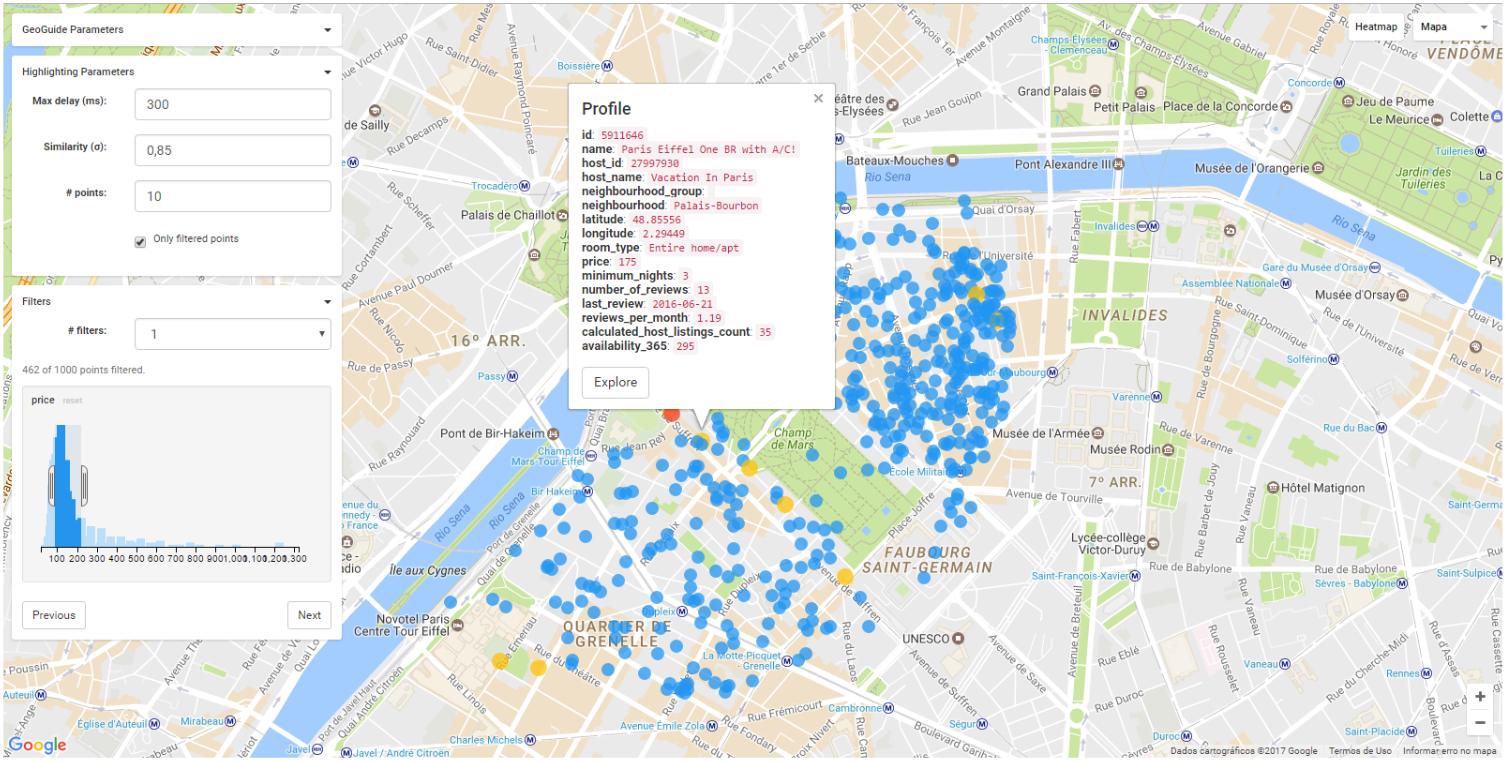
\includegraphics[width=\textwidth]{images/geoguide-example-airbnb}
	\caption{GeoGuide Image on Airbnb Dataset - Paris City}
	\label{fig:geoguide-example-airbnb}
	\vspace{-10pt}
\end{figure*}

\subsection{Outliers}

% TODO: usar definição de Hawkins (procurar slide dos algoritmos de detecção de outlier)
% TODO: adicionar exemplos de outlier detection

Outliers in the statistics area are when one finds ``aberrant values'' in a given series of data, that is when one finds an atypical value or with a great distance from the normal distribution in that set. For example, when a researcher wants to monitor the temperature of his CPU during a certain time interval and it has been realized that the temperature range is between 34 ºC and 45 ºC degrees being 48 ºC the maximum temperature and 27 ºC the minimum temperature and in the middle of this sample are some punctual registers of 0 ºC, this can be characterized as an outlier and, most likely, will be understood as a malfunction of the equipment that performed the collection of these CPU temperatures.

However, there are several ways to interpret an Outlier (not only as a collection error), but also as: data that belong to a different population of the sample, a damaged data, areas in which a certain theory is not valid or even, when the sample is too large, it is normal to have some small amounts of outliers in that group. In cases where it is proven that it is not the fault of a collection equipment malfunction or that it was not a human mistake, it is extremely important to know the why of that outlier and try to understand it, because it is not interesting for a research simply remove it from the sample or re-signify it by assigning a new value. This change may compromise the validity of the research, and if this is done, it is extremely important to document and record those changes.

As the information technologies improve and continuously increase their computational power, a great variety of algorithms for outlier detection has been surging and applied in different contexts with diverse characteristics and the choice for one of those algorithms is based on the problem domain. Next section will present some of those algorithms with a brief explanation about each one.

\section{Algorithms}

\subsection{Z-Score}

Z-Score is one of the simplest methods for detecting outliers in a dataset. It is a
parametric method and takes into account only one attribute per execution. It is also
necessary the input of a threshold (usually is a value between 2.5 to 3.5) to be able
to define if a given data can be considered an outlier or not. This method is suitable
for small datasets that follow the Gaussian distribution.

\subsection{DBSCAN}

It is a density-based spatial clustering algorithm \cite{Ester:1996:DAD:3001460.3001507} that can be applied in datasets that cannot be presumed what their distribution. It accepts multidimensional datasets (with 3 or more dimensions). However, you need a parameter (MinPts) that defines how many minimum points are needed to form a cluster. Thus, if the size of the set change, this parameter will need to be updated, otherwise the DBSCAN can become inefficient.

\subsection{Isolation Forests}

It is an algorithm of detection of outliers \cite{IsolationForests} that uses a concept of machine learning that
is the decision tree. It is one-dimensional (only takes one attribute at a time) and is
required few parameters (this facilitates the configuration and use of the algorithm).
No need to climb your values and a very robust algorithm for large datasets.

% \subsection{ISODEPTH}

% TODO: IDSODEPTH

\subsection{FDC}

It is a depth-based algorithm \cite{Johnson:1998:FCD:3000292.3000332} approach for detection of outliers in 2D datasets based on the concept of ISODEPTH algorithm. The FDC computes the first k 2D depth contours (the points that can be considered outliers) by restricting to a small part of the complete dataset. In this way, it is more efficient by not having to calculate in the complete dataset and thus scaling more easily for large datasets of two dimensions.

\subsection{HOD}

It is a distance-based outlier detection method \cite{Xu2016} that emerges to overcome the statistics-based
concept because in the vast majority of datasets the probability distribution is not known.
In this way, the method search for outliers based on their distance from their neighbors
and if that point has a distance greater than a predefined parameter, then that point is
considered an outlier. However, if there is a cluster of outliers in the dataset, this
can affect its detection by distance-based algorithms, with this comes the concept of HOD
(Hidden Outlier Detection) algorithms that aim to find outliers even when they are grouped
and in enough quantity to form a cluster.

% \subsection{Nested Loop}

% TODO: Nested Loop

\subsection{ORCA}

It is a distance-based algorithm \cite{Bay:2003:MDO:956750.956758} that optimizes a simple nested loop algorithm (which are logarithmic algorithms and extremely inefficient when dealing with large datasets) by removing possible non-outliers during their execution. This way, instead of processing the complete dataset by calculating all possible distances, it removes unnecessary calculations that would be executed if a non-outlier point were taken to the end. From him, new researches have emerged further refining this concept.

\subsection{Linearization}

It is a distance-based algorithm \cite{10.1007/3-540-45681-3_2} that detects outliers by calculating the sum of the distances
of a point in relation to its neighbor, calling it weight, and setting an outlier as the points
with the greatest weights in the dataset. In this way, it is an efficient algorithm and it is
linearly scaled both in the number of points and in the number of dimensions. To calculate these
outliers more efficiently the algorithm uses the concept of the Hilbert space-filling curve.

\subsection{RBRP}

It is an algorithm for high-performance multidimensional datasets that is based on distances between the points to be able to define what the outliers are \cite{Ghoting2006}. Its difference to the other distance-based algorithms is that it is more efficient for datasets with multiple dimensions and in comparisons with others, its scalability is approximately linear for the number of dimensions and logarithmic for the number of points in the dataset.

\subsection{LOF}

It is a density-based algorithm that adds a new concept in the search for outliers: the
Local Outlier Factor (LOF) \cite{Breunig:2000:LID:335191.335388}, which is a degree of propensity to be an outlier so that the
process of outlier definition is not more binary, but something gradual. With this, the
approach is not to define whether a point is an outlier or not, but rather the ``how outlier''
that point is in that dataset. The outlier factor is local in the sense that only a neighborhood
of that point is taken into account to define its factor.

% \subsection{INFLO}

% TODO: INFLO

% \subsection{LOCI}

% TODO: LOCI

\subsection{ABOD}

It is an angle-based algorithm \cite{Kriegel:2008:AOD:1401890.1401946} for detection of outliers that is focused on high-dimensional datasets, different from other distance-based algorithms that end up damaged when one has many dimensions. Your approach is based on the calculation of a degree of angle between the different vectors of a point with its neighbors. With this, more centralized points within the cluster will have this degree calculated with a high value, the points more on the edge of the clusters will have this degree a little smaller and the possible outliers will have that degree with a very small value, since they will generally be far from the cluster in a particular direction.

% \subsection{SOD}

% TODO: SOD

\vspace{25pt}

Based on the algorithms presented, we organize each one according the answer of proposed questions about outlier detection algorithms in general. The proposed questions are: \textbf{I} \textit{Is it parametric?}; \textbf{II} \textit{Which is the approach?}; \textbf{III} \textit{Is it scalable in performance terms?}; \textbf{IV} \textit{Is it multidimensional scalable?} and \textbf{V} \textit{Does it receive any argument?}. The result is presented in the Table \ref{table:algorithms-comparison}.

\begin{table}[]
	\centering
	\begin{tabular}{|l|l|l|l|l|l|}
		\hline
		\textbf{Algorithms}               & \textbf{I} & \textbf{II}      & \textbf{III} & \textbf{IV} & \textbf{V} \\ \hline
		\textbf{Z-Score}                  & Yes        & Model Based      & No           & No          & Yes        \\ \hline
		\textbf{DBSCAN}                   & No         & Density Based    & No           & Yes         & Yes        \\ \hline
		\textbf{Isolation Forests}        & No         & Depth Based      & No           & No          & No         \\ \hline
		\textbf{FDC}                      & No         & Depth Based      & Yes          & No          & No         \\ \hline
		\textbf{Hidden Outlier Detection} & No         & Distance Based   & Yes          & Yes         & Yes        \\ \hline
		\textbf{ORCA}                     & No         & Distance Based   & No           & Yes         & Yes        \\ \hline
		\textbf{Linearization}            & No         & Distance Based   & Yes          & Yes         & Yes        \\ \hline
		\textbf{RBRP}                     & No         & Distance Based   & Yes          & Yes         & Yes        \\ \hline
		\textbf{LOF}                      & No         & Density Based    & No           & Yes         & Yes        \\ \hline
		\textbf{ABOD}                     & No         & High Dimensional & No           & Yes         & No         \\ \hline
	\end{tabular}
	\caption{Comparison of the presented Outlier Detection Algorithms}
	\label{table:algorithms-comparison}
\end{table}

Each question has a specific reason to be in the Table \ref{table:algorithms-comparison}. The question \textbf{I} is about the probability distribution of the dataset. If the algorithm is parametric, so we can assume a probability distribution based on a fixed set of parameters. The question \textbf{II} serves to classify each algorithm based on his approach for detect a data as an outlier or not, the options are: \textit{Model Based}, \textit{Density Based}, \textit{Depth Based}, \textit{Distance Based}, \textit{High Dimensional}. The question \textbf{III} is relative to the performance of each algorithm, if the algorithm execution time is not compromised as the input data increase, it means the algorithm is scalable in perfomance terms. The question \textbf{IV} is about the performance of each algorithm too, but in this case is related to the perfomance when the dimension of the data increase. At least, the question \textbf{V} indicates if the algorithm require any input argument to process the dataset, this is important because if it requires many arguments, this can be a accuraccy problem when the dataset increase.